% Deck E: Revision 1: status and product plan; all provenance is in speaker notes.
% WBR advisor progress report -- evidence snapshot 2026-10-13.
% Build: latexmk -xelatex main.tex   (see README.md)
% Content sources and number provenance: SOURCES.md.
% Historical Pi measurements are labeled MEASURED; calculations, assumptions,
% published comparisons, plans and OPEN qualification remain distinct.
\documentclass[aspectratio=169,12pt,t]{beamer}

% Speaker notes: uncomment ONE line to see them.
% \setbeameroption{show notes on second screen=right}  % dual-screen (pdfpc)
% \setbeameroption{show only notes}                     % notes handout

\usetheme[progressbar=none, sectionpage=none]{moloch}
% A 208 x 117 mm canvas retains 16:9 and the actual 12pt class fonts.
% Long owner-approved sentences fit without frame scaling or reduced fonts.
\geometry{paperwidth=208mm,paperheight=117mm}

% ---------- fonts ----------
\usepackage{fontspec}
\setsansfont{Avenir Next}[BoldFont={Avenir Next Demi Bold}]
\setmonofont{Menlo}[Scale=1.0]
\newcommand{\captiontype}{\small}

% ---------- palette ----------
\definecolor{navy}{HTML}{1F3A5F}
\definecolor{teal}{HTML}{2A9D8F}
\definecolor{fault}{HTML}{E76F51}
\definecolor{paper}{HTML}{FAFAF7}
\definecolor{ink}{HTML}{22262B}
\definecolor{muted}{HTML}{6B7280}
\definecolor{rule}{HTML}{D6D9DE}

\setbeamercolor{normal text}{fg=ink, bg=paper}
\setbeamercolor{frametitle}{fg=paper, bg=navy}
\setbeamercolor{progress bar}{fg=teal, bg=rule}
\setbeamercolor{alerted text}{fg=fault}
\setbeamercolor{example text}{fg=teal}
\setbeamercolor{structure}{fg=navy}
\setbeamercolor{title separator}{fg=teal}
\setbeamercolor{footline}{fg=muted}
% Beamer otherwise inherits the fault/alert color for in-slide citations.
\setbeamercolor{bibliography entry author}{fg=navy}
\setbeamercolor{bibliography entry title}{fg=ink}
\setbeamercolor{bibliography entry location}{fg=muted}
\setbeamercolor{bibliography entry note}{fg=muted}
\setbeamercolor{block title}{fg=paper, bg=navy}
\setbeamercolor{block body}{bg=navy!6}
\setbeamerfont{frametitle}{size=\large, series=\bfseries}
\setbeamertemplate{frametitle}{\nointerlineskip\begin{beamercolorbox}[wd=\paperwidth,sep=2mm,leftskip=4mm]{frametitle}\usebeamerfont{frametitle}\insertframetitle\strut\end{beamercolorbox}}
\setbeamertemplate{itemize items}{\color{teal}\rule[0.25ex]{0.45em}{0.45em}}
\setbeamertemplate{bibliography item}[text]
\setbeamertemplate{page number in head/foot}[totalframenumber]
\hypersetup{colorlinks=true, linkcolor=navy, urlcolor=navy, citecolor=navy}
% Keep the appendix bookmark free of Beamer translation commands.
\pdfstringdefDisableCommands{\def\translate#1{#1}}

\setbeamertemplate{itemize subitem}{\color{muted}--}

% ---------- packages ----------
\usepackage{tikz}
\usetikzlibrary{arrows.meta, positioning, automata, calc, shapes.geometric, fit, backgrounds, decorations.pathreplacing}
\usepackage{booktabs}
\usepackage{array}
\newcolumntype{L}[1]{>{\raggedright\arraybackslash}p{#1}}
\usepackage{amsmath}
\usepackage{siunitx}
\sisetup{detect-all}

% ---------- helpers ----------
\newcommand{\muted}[1]{{\color{muted}#1}}

% \slideimg[<max height>]{<width>}{<V-id>}{<caption for placeholder>}
% Shows images/<V-id>.jpg or .png if present, otherwise a labelled gray box of the same size.
\newcommand{\slideimg}[4][0.64\textheight]{%
  \IfFileExists{images/#3.jpg}{%
    \includegraphics[width=#2, height=#1, keepaspectratio]{images/#3.jpg}%
  }{\IfFileExists{images/#3.png}{%
    \includegraphics[width=#2, height=#1, keepaspectratio]{images/#3.png}%
  }{%
    \begin{tikzpicture}
      \node[draw=rule, fill=black!6, rounded corners=2pt, minimum width=\dimexpr#2-1pt\relax, outer sep=0pt,
            minimum height=#1, align=center, text width=\dimexpr#2-8mm\relax, font=\small, text=muted]
        {\textbf{#3}\\[2pt]#4\\[2pt]\small Illustration pending};
    \end{tikzpicture}%
  }}%
}

\tikzset{
  box/.style={draw=navy, fill=white, rounded corners=2pt, align=center, font=\small,
              minimum height=7mm, inner sep=3pt},
  flow/.style={-{Stealth[length=2mm]}, thick, color=navy},
  faultflow/.style={-{Stealth[length=2mm]}, thick, color=fault},
  lbl/.style={font=\small, color=ink, fill=paper, inner sep=1pt},
}

% Only the page number appears in the footer.
\setbeamerfont{footline}{size=\small}
\setbeamertemplate{footline}{\hbox{\begin{beamercolorbox}[wd=\paperwidth,ht=4mm,dp=1mm,rightskip=6mm]{footline}\hfill\insertframenumber/\inserttotalframenumber\end{beamercolorbox}}}
\AtBeginSection{\begin{frame}[c]\centering{\Huge\bfseries\color{navy}\thesection. \insertsectionhead\par}\end{frame}}
\setbeamertemplate{navigation symbols}{}
\setbeamersize{text margin left=6mm,text margin right=6mm}
\setlength{\tabcolsep}{4pt}
\renewcommand{\arraystretch}{1.02}
\title{WBR Perception: Progress Report}
\subtitle{Known baseline before camera adaptation}
\author{}
\institute{}
\date{13 October 2026}


\newcounter{slidefigure}
\newcommand{\figcap}[1]{\par\smallskip{\centering\captiontype\color{muted}\refstepcounter{slidefigure}Figure \theslidefigure: #1\par}}
\newcommand{\figagain}[1]{\par\smallskip{\centering\captiontype\color{muted}Figure~\ref{fig:#1}: \csuse{caption#1}\par}}
\setbeamerfont{bibliography entry author}{size=\normalsize}
\setbeamerfont{bibliography entry title}{size=\normalsize}
\setbeamerfont{bibliography entry location}{size=\normalsize}
\setbeamerfont{bibliography entry note}{size=\normalsize}
\setlength{\emergencystretch}{2em}
\setbeamerfont{normal text}{size=\normalsize}
\setbeamerfont{itemize/enumerate body}{size=\normalsize}
\setbeamerfont{itemize/enumerate subbody}{size=\normalsize}
\linespread{1.12}
\AtBeginDocument{\setlength{\leftmargini}{1.1em}\setlength{\leftmarginii}{1.2em}\setlength{\labelsep}{.35em}}
\newcommand{\namedcap}[2]{\figcap{#2}}
% Apply spacing after Beamer has created each list (including nested lists).
\usepackage{etoolbox}
\makeatletter
\apptocmd{\itemize}{\ifnum\@itemdepth=1\setlength{\itemsep}{.55em}\else\setlength{\itemsep}{.25em}\fi\setlength{\parsep}{0pt}\setlength{\parskip}{0pt}\setlength{\topsep}{0pt}}{}{}
\makeatother
\newsavebox{\figurebox}
\newcommand{\fig}[3][.48\textheight]{%
  \ifcsdef{diagram#2}{\sbox{\figurebox}{\csuse{diagram#2}}}{%
    \sbox{\figurebox}{\includegraphics[width=\linewidth,height=#1,keepaspectratio]{images/#2.jpg}}}%
  \par\centering\begin{minipage}{\wd\figurebox}\centering
  \usebox{\figurebox}%
  \ifcsdef{assetcaption#2}{\csuse{assetcaption#2}}{%
    \csgdef{assetcaption#2}{\repeatassetcap{#2}}%
    \csgdef{assettext#2}{#3}\figcap{#3}%
    \csxdef{assetnumber#2}{\theslidefigure}}\end{minipage}\par}
\newcommand{\repeatassetcap}[1]{\par\smallskip{\centering\captiontype\color{muted}%
  \begingroup\renewcommand{\label}[1]{}Figure \csuse{assetnumber#1}: \csuse{assettext#1}\par\endgroup}}
\makeatletter
\newcommand{\takeaway}[1]{\global\beamer@framebottomskip=0pt\par\medskip\begin{beamercolorbox}[wd=\linewidth,sep=0pt]{block body}%
  \begin{tabular}{@{}!{\color{teal}\vrule width 3pt}p{\dimexpr\linewidth-22pt\relax}@{}}\normalsize\strut #1\strut\end{tabular}%
  \end{beamercolorbox}\par}
\makeatother


% Course additions retain the approved palette, canvas, type and figure system.
\newcommand{\evidence}[1]{{\small\bfseries\color{teal!70!black}#1}\par\medskip}
\newcommand{\coursefigure}[3]{\begin{minipage}{\linewidth}\centering#2\figcap{\label{fig:#1}#3}\end{minipage}}



\newcommand{\deckitems}[1]{\begin{itemize}#1\end{itemize}}
\newcommand{\deckflow}[1]{\begin{tikzpicture}[node distance=9mm]
\foreach \txt [count=\i] in {#1}{\node[box,font=\normalsize,text width=33mm,minimum height=14mm] (n\i) at ({mod(\i-1,4)*4.7},{-floor((\i-1)/4)*2.4}) {\txt};}
\end{tikzpicture}}


\newcommand{\src}[1]{\note{Source: \detokenize{#1}}}
\title{WBR perception — status report, 14 October 2026}
\date{14 October 2026}
\begin{document}
\raggedright

\begin{frame}[c]\relax
{\huge\bfseries\color{navy}WBR perception — status report,\par 14 October 2026\par}
\medskip{\color{teal}\hrule height .6pt}\bigskip
\begin{columns}[c,onlytextwidth]
\begin{column}{.60\textwidth}
\Large Our next product milestone is a D435i visual-inertial demo on the Raspberry Pi 5.\par\bigskip
\normalsize The artificial intelligence (AI) team reports to you as the project owner.\par\medskip
\muted{WBR means wheel-biped robot.}
\end{column}
\begin{column}{.35\textwidth}
\slideimg[.36\textheight]{\linewidth}{P04}{D435i camera}
\par\small\muted{The illustration makes no validation claim.}
\end{column}
\end{columns}
\src{experiments/2026-10-14-SESSION_FACTS_ADDENDUM.md; slides_report/main.tex}
\note{Target duration: five minutes for eleven slides. All hardware observations are historical source facts, not newly executed tests. P04 is reused from slides_course/images/P04.png.}
\end{frame}


\begin{frame}{The input works briefly; the camera-to-plot chain is unfinished.}
\centering
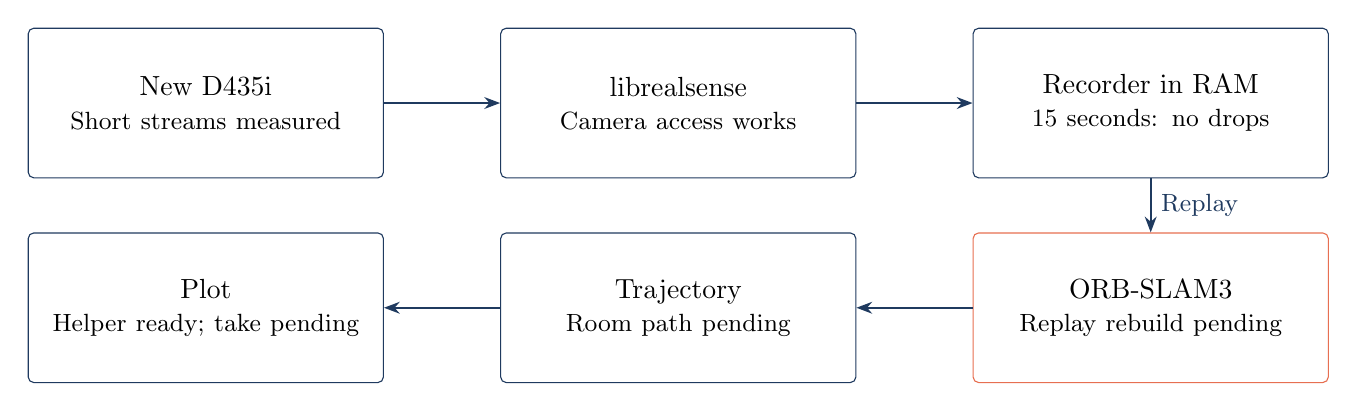
\begin{tikzpicture}[x=1cm,y=1cm,stage/.style={box,text width=43mm,minimum height=19mm,font=\normalsize}]
\node[stage] (cam) at (0,0) {New D435i\\\small Short streams measured};
\node[stage] (sdk) at (6,0) {librealsense\\\small Camera access works};
\node[stage] (ram) at (12,0) {Recorder in RAM\\\small 15 seconds: no drops};
\node[stage,draw=fault] (orb) at (12,-2.6) {ORB-SLAM3\\\small Replay rebuild pending};
\node[stage] (traj) at (6,-2.6) {Trajectory\\\small Room path pending};
\node[stage] (plot) at (0,-2.6) {Plot\\\small Helper ready; take pending};
\draw[flow] (cam)--(sdk); \draw[flow] (sdk)--(ram);
\draw[flow] (ram)--node[right,font=\small]{Replay}(orb);
\draw[flow] (orb)--(traj); \draw[flow] (traj)--(plot);
\end{tikzpicture}
\par\medskip\raggedright\small RAM means random-access memory; SLAM means simultaneous localization and mapping.\par\medskip
\normalsize The later STM32H7 controller owns balance and motor safety; this demo produces a path only.
\src{experiments/2026-10-13-SESSION_FACTS_FOR_SLIDES.md section E; experiments/2026-10-14-SESSION_FACTS_ADDENDUM.md items 2,4,5,8; AGENTS.md}
\note{Diagram is the record/replay route on the Pi; plotting is on the Mac after transfer. Live input bypasses the recorder through librealsense. Recorder and live program never run concurrently. STM32H7 is a controller-family/series name. No architecture is changed.}
\end{frame}
\begin{frame}{Three EuRoC runs match the published accuracy range.}
\begin{columns}[T,onlytextwidth]
\begin{column}{.43\textwidth}
{\Huge\bfseries\color{teal}3.7–4.2 cm\par}\medskip
\large Our absolute trajectory error (ATE) was close to the paper's \textbf{3.6 cm}.\par\bigskip
\normalsize Relative pose error (RPE) was about \textbf{1.3 cm over one second}.
\end{column}
\begin{column}{.52\textwidth}
\deckitems{
\item The public EuRoC machine-hall dataset provides a known reference path.
\item The native build reproduces similar accuracy on this sequence.
\item This does not prove D435i calibration or real-time speed.
\item The 8-gigabyte (GB) Pi rerun is still pending.}
\end{column}
\end{columns}
\src{experiments/2026-10-13-n4a-euroc-mh01/REPORT.md; slides_course/qa/n4a-traj-eval-summary.md; experiments/2026-10-14-SESSION_FACTS_ADDENDUM.md}
\note{ATE root-mean-square values with rigid rotation/translation alignment and no scale: 0.041461, 0.036844, 0.041604 m. Paper comparison is approximately 0.036 m, Table II, MH01; paper reports a median of ten runs, not our three-run statistic. Translational RPE at a one-second interval: 0.013295, 0.013559, 0.014021 m; mean 0.013625 m. The brief requests about 1.3 cm; individual values span roughly 1.3-1.4 cm. Benchmark was on the 4 GB Pi under under-voltage, so timing is invalid. No 8 GB rerun results appear in the permitted sources.}
\end{frame}


\begin{frame}{Memory recording fixes short-test drops; the long take is pending.}
\large
\deckitems{
\item The 20-second still take delivered both infrared (IR) streams at 30 hertz (Hz) and inertial measurement unit (IMU) data, with a shutdown gap.
\item The first 100-second moving take was unusable: 0.3–2.9-second gaps recurred about every five seconds.
\item Card writes reached 16.6 megabytes per second (MB/s), below the 18.4 MB/s input; slow storage is the strongly inferred cause.
\item Recording into RAM first gave 15 seconds with zero dropped frames and a 33-millisecond maximum gap.}
\vfill\takeaway{A 100-second take of about 1.7 GB fits in the 8 GB Pi; it has not yet been measured.}
\src{experiments/2026-10-14-SESSION_FACTS_ADDENDUM.md items 1-4}
\note{Still take: about 19 seconds correct then a 0.7-second shutdown gap. Long-take gaps began after 22 seconds. RAM IR rate 29.99 Hz; gyro 200.2 Hz; accel 101 Hz; copy checksum verified. Memory-backed area was 3.9 GB. Diagnostic observations, not gate passes.}
\end{frame}

\begin{frame}{The replay fix needs rebuilding, and lab readiness is unresolved.}
\large
\deckitems{
\item The native build needed three compatibility patches; a fourth fixes the camera replay's first-frame crash from an uninitialized pointer.
\item Power loss interrupted that rebuild; the 8 GB Pi boots with the same 32 GB card but still has under-voltage.
\item Ethernet is loose and Wi-Fi is unseen on this board; the 128 GB card still needs qualification.
\item The 64 GB Universal Serial Bus (USB) stick writes only about 1 MB/s; calibration is also unfinished.}
\vfill\takeaway{Next we unblock the lab session, finish the rebuild, and test one complete camera-to-plot route.}
\src{experiments/2026-10-13-SESSION_FACTS_FOR_SLIDES.md sections A,C; experiments/2026-10-14-SESSION_FACTS_ADDENDUM.md items 1,5-7}
\note{Patch four is applied in the isolated Pi build copy; three of about 27 library objects rebuilt before power loss. Wi-Fi worked on 4 GB, not seen on 8 GB within seven minutes; cause unknown. Stick measured 1.09 MB/s. Supply ordered 5.1 V/5 A. Calibration nominal, noise assumed, offset unknown; warning retained.}
\end{frame}

\begin{frame}{First, a prepared lab session makes the remaining tests possible.}
\large
\deckitems{
\item \textbf{Why:} power, connectivity and fresh-camera entry checks determine whether we can proceed.
\item \textbf{You:} confirm the 15 October slot, bring the 8 GB Pi and camera, secure Ethernet or arrange Wi-Fi, and confirm the 5-ampere (A) supply's availability.
\item \textbf{Team:} check the setup and follow N1, N2 and N3 in order; the mandatory 300-second raw-input soak is retained.
\item \textbf{Done:} the correct Pi is reachable and entry evidence is reviewed; unmet conditions keep progression blocked.}
\vfill\takeaway{At the bench, you must explicitly confirm camera availability before any camera or SLAM execution.}
\src{experiments/2026-10-14-lab-prep/LAB_RUNBOOK_2026-10-15.md one-page checklist; experiments/2026-10-14-SESSION_FACTS_ADDENDUM.md items 1,7}
\note{Exact authorization: CAMERA AVAILABLE. N1-N3 are gate names. N1 USB >=5000M. N2 exact raw IR1 Y8 640x480/15, gyro/200, accel/100; 20/105/300 seconds, mandatory soak and unchanged timing/health criteria. N3 evidence review. Diagnostic override never becomes PASS; under-voltage can block acceptance. 100-second stereo/30 demo does not replace gates. Camera direct blue USB3 port; Pi and connectors fixed, cable slack. Role split proposed, not evidenced named ownership.}
\end{frame}

\begin{frame}{Second, finishing the rebuild lets us retest the crash fix.}
\large
\deckitems{
\item \textbf{Why:} camera replay failed before producing a usable trajectory; the applied fix is not yet in a completed build.
\item \textbf{Team:} resume the interrupted build on the 8 GB Pi and check the example uses the rebuilt library.
\item \textbf{You:} keep the Pi powered and the lab connection available while the team checks the result.
\item \textbf{Done:} the build finishes successfully and library linkage is verified, before capture and replay.}
\src{experiments/2026-10-14-SESSION_FACTS_ADDENDUM.md item 5; experiments/2026-10-14-lab-prep/LAB_RUNBOOK_2026-10-15.md rebuild checklist}
\note{No duration promised: remaining build time unknown. Keep logs and stop on failure. Do not reapply patch or reset checkout. Build success alone does not establish replay fixed.}
\end{frame}

\begin{frame}{Third, a full memory take gives us repeatable camera input.}
\large
\deckitems{
\item \textbf{Why:} replaying the same take separates input faults from SLAM faults without repeating every camera movement.
\item \textbf{You:} move the camera smoothly for 100 seconds, translating within 1–2 seconds, then make a small loop and finish 5–10 seconds still.
\item \textbf{Team:} record into RAM, copy afterwards, and audit both image streams, motion data, timestamps and power.
\item \textbf{Done:} recording and copy checks succeed, rates are as expected, and no unexplained gaps remain; otherwise review before replay.}
\vfill\takeaway{Keep the Pi and cables fixed; recheck memory and free space before the take.}
\src{experiments/2026-10-14-lab-prep/LAB_RUNBOOK_2026-10-15.md capture checklist; experiments/2026-10-14-SESSION_FACTS_ADDENDUM.md items 3,4}
\note{First 20-30 seconds: translate 10-30 cm all axes, gentle +/-15-30 degree rotations. Well-lit textured static scene, emitter off. Stereo 640x480 Y8/30, gyro/200, accel/100 Hz. Recorder only camera owner. Audit ordered/common-domain stamps, beginning/end exclusions, kernel/power logs, checksum. Acquisition local Pi. Card staging not qualified dataset storage.}
\end{frame}

\begin{frame}{Fourth, replay and a plot show whether tracking holds together.}
\large
\deckitems{
\item \textbf{Why:} offline replay lets us inspect initialization, tracking and resets before a live attempt.
\item \textbf{Team:} replay the reviewed take on the Pi, then copy and verify the outputs and plot the trajectory on the Mac.
\item \textbf{You:} review the result with the team before agreeing to the live attempt.
\item \textbf{Done:} initialization, sustained tracking, one stable map and nonempty trajectories agree with the logs; failures trigger investigation.}
\vfill\takeaway{A plausible room plot cannot establish accuracy because there is no reference path.}
\src{experiments/2026-10-14-lab-prep/LAB_RUNBOOK_2026-10-15.md review-replay-plot and Mac plotting; experiments/2026-10-14-SESSION_FACTS_ADDENDUM.md item 8}
\note{Review actual map IDs, resets, counters and tracking state 2, not creation-message counts or largest-map export alone. Retain failures. Offline wall duration is not live throughput. Plot helper checked against EuRoC does not imply successful D435i replay. Live depends on runbook prerequisites.}
\end{frame}

\begin{frame}{Fifth, a reviewed live attempt completes the diagnostic demo.}
\large
\deckitems{
\item \textbf{Why:} live input tests the final connection from the physical camera to SLAM after replay has been reviewed.
\item \textbf{You:} remain at the bench and repeat the smooth camera motion, keeping the Pi and connectors stationary.
\item \textbf{Team:} run the same binary and settings on live input for 90 seconds, inspect tracking and power, then verify shutdown and saved outputs.
\item \textbf{Done:} retained logs and a trajectory support a one-slide summary of what worked, what failed and what remains unproven.}
\vfill\takeaway{Run live only after offline review; record failures as outcomes and keep their evidence.}
\src{experiments/2026-10-14-lab-prep/LAB_RUNBOOK_2026-10-15.md live checklist and command card; experiments/2026-10-14-SESSION_FACTS_ADDENDUM.md shortest path}
\note{90-second attempt plus 30-second shutdown allowance in command card. Timeout not success: inspect finalization, counters/backlog and health; forced kill or missing finalization fails. Never run recorder concurrently. Copy immediately to new Mac destination and verify; preserve calibration warnings. Summary is future deliverable.}
\end{frame}

\begin{frame}{The demo is a milestone; reliable product behavior comes next.}
\large
\deckitems{
\item \textbf{If successful,} the demo shows the D435i-to-trajectory route working on the Pi 5 for the reviewed attempts.
\item It does not establish room accuracy, calibrated sensing, sustained real-time speed or motor and jump safety.
\item \textbf{You provide:} stable 5 A power, the 128 GB card for qualification, and a further lab slot for calibration and repeat tests.
\item \textbf{Team then verifies:} power and storage, camera–IMU calibration, and fresh N1–N3 evidence before claiming readiness.}
\vfill\takeaway{The next decision is lab and hardware availability; acceptance still requires observed results.}
\src{experiments/2026-10-14-SESSION_FACTS_ADDENDUM.md shortest path; experiments/2026-10-14-lab-prep/LAB_RUNBOOK_2026-10-15.md; experiments/2026-10-13-SESSION_FACTS_FOR_SLIDES.md sections A,E,F; AGENTS.md}
\note{Entry gates still required before demo: follow-up repeats under stable power and calibration, not permission to bypass. Exact USB/raw/20-105-300-second soak/timing-health requirements unchanged. Reference trajectory needed for accuracy; stable-power live measurements for speed. STM32H7 owns hard-real-time and motor/jump safety. No delivery dates, lab duration estimates or passes invented.}
\end{frame}
\end{document}
